\section{為什麼特首選舉會被批評為假選舉?}

目前香港特區的行政長官並非由香港人一人一票選出,而是由一個1,200人的選舉委員會產生。選舉委員會一般於行政長官選舉前約三個月產生(在特區早年曾有例外),再由選舉委員會提名和投票產生行政長官人選,然後提交中央政府任命。不過全港五百多萬名合資格選民當中,只有二十多萬人可以在選舉委員會選舉中投票選出他們的代表。由於選舉委員會本身欠缺代表性,所以整個行政長官選舉也被認為是毫無代表性,嚴重拖低其認授,甚至被認定為是假選舉。

選舉委員會除了產生的基礎狹窄,還有嚴重的票值不均等問題。所謂票值均等,是次每位投票者對選舉結果的影響力不應該差距大遠。例如香港的區議會選舉規定約每16,964名居民劃為一個選區,選出一名區議員。現實上人口最少的選區只有六千人,最多的選區卻有二萬六千多人,住在人口較多選區的居民就會覺得不公平了。

選舉委員會的1,200名委員名額並不是平均分配給二十多萬名可投票的選民的。選舉委員會分四個界別,分別由商界、專業、社會和政界代表擔任,當中不同組別所得的代表數目和其選民基礎差距極大,而且可謂毫無準則可言。例如代表中小學教師的教育界有80,643人有權投票,可選出30個選舉委員;與此同時,漁農界只有154人有權投票,卻可選出60個選舉委員。無論從人數、經濟、或社會貢獻出發,也難以解釋漁農界為何在選委會當中會比教師有多一倍的席位。

\begin{figure}[htbp]
    \centering
    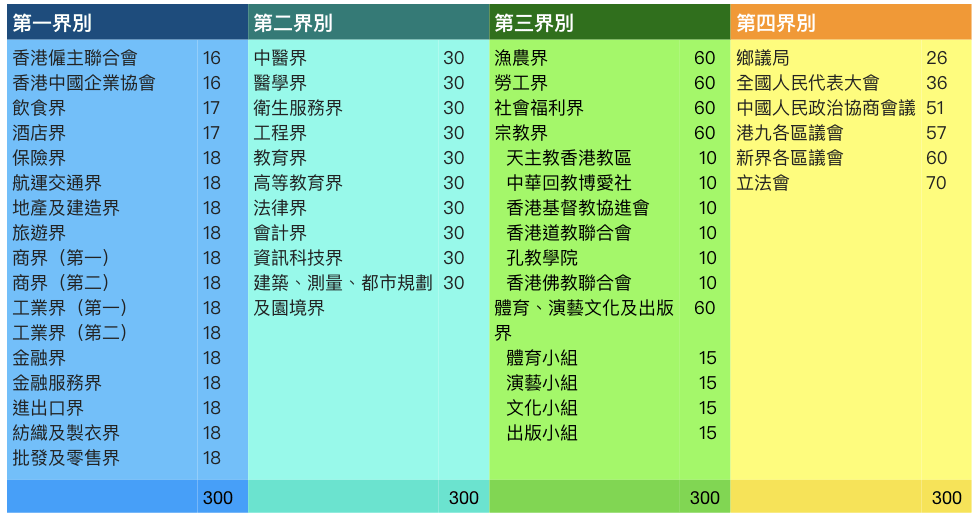
\includegraphics[width=0.7\textwidth]{c18/h-klesson1-025.png}
    \caption{選舉委員會的席位分配} 
\end{figure}

與此同時,誰有權成為不同組別的投票人也是沒有準則的。有些組別例如會計界,只要是註冊會計師就可以投票,全港近三萬名名會計從業員中有26,001人是選民。但到了保險界,卻只有保險公司的東主才可以投票,於是全港近五萬名的保險從業員都沒有投票權,只有131名東主是選民。至於為什麼會計界和保險界有不同做法,是沒有解釋的。回到剛才提到的漁農界,那154人和現役漁民或農民不一定有關,也不是由他們所選出,而是由規定的一系列漁農業團體作為代表。至於為什麼是這些團體而不是另一些團體,這些團體是否有代表性,新成立的團體要怎樣才可能為被指定的團體,同樣是沒有解釋的。

% \begin{figure}[ht!]
%     \centering
%     \includemedia[
%     width=0.6\linewidth,height=0.45\linewidth,
%     activate=pageopen,
%     flashvars={
%         modestbranding=1  % no YT logo in control bar
%         &autohide=1       % controlbar autohide
%         &showinfo=0       % no title and other info before start
%     }
%     ]{}{https://youtu.be/tCd17uhOKr8}   % Flash file
%     \caption{《小圈子篇》 真普選聯盟製作 2014}
% \end{figure}

由於在許多商界組別當中,投票人很多時候都以公司為單位,於是便出現某些大企業可以通過其關係企業座擁多票的情況。舉個例,僱主聯合會在選委會當中佔16席,由139名投票人產生。按傳媒統計,全港六大地產商加起來已佔三分之一的票數,很有能力左右誰能成為該界別的選委。事實上,在二零一六年選出的僱主聯合會代表,全數均為在沒有競爭之下自動當選的。

與此同時,由於在某些組別當中只要是合資格的團體或公司便可投票選出選舉委員,有意各逐的參選人可以預先安排友好人士大舉成立相關團體或公司,實行種票。廉政公署就曾經揭發數十名沒有資訊科技學歷或經驗的市民,收取金錢報酬註冊成為資訊科技界專業團體的會員,進而成為資訊科技界功能界別的選民。

既然選舉委員會的制度有這麼多的漏洞,為何至今仍然會被用作為選舉行政長官的方法?學術界的答案是這個方法可以很有效地確保中央政府屬意的候選人當選,同時又擺出「港人治港」的模樣來延緩對真正普選的訴求,容許中央政府可以聲稱行政長官是由香港人選出來(儘管這些香港人如何投票很大程度上受中央政府左右)。

分析1,200個選委席位的選舉方法,可見各種限制成為投票人資格的招數,確保大多數的選委都聽命於中央政府。其中來自商界的選委,由於他們本身在中國大陸有千絲萬縷的利益關係,無論自願或被迫,都會支持中央政府屬意的行政長官候選人。扣除選民資格本身有限的「團體票」和商界選委後,可供一般市民競逐的選委席次不足一半。由於法例規定候選人必須要有超過一半的選委支持才能當選,也就是說一般市民要透過競逐選委來決定新一任行政長官的人選,和追逐奇蹟無異。

過去多次行政長官選舉都可看到它如何受中央政府操控。在一九九六年的首屆行政長官選舉前,時任中共總書記江澤民在北京會見香港特區籌委會,刻意在人群中尋找董建華與他握手,外界普遍認為是要向在場人士表明董建華已受到政治上的祝福。到了二零零二年的特首選舉,「欽點」的情況變得更赤裸裸。當時規定的選委人數是800人,而最少要有100名選委提名才可成為正式候選人。結果董建華一個人就拿了714名選委的提名,變相等於不可能有其他人參選和他競爭。這種情況帶來了一個很危險的後果:本來香港的選舉都是不記名的,選民進入投票間之後如何在選票上面蓋章,只有他自己一個人知道。投票保密是民主制度的重要原則,可以確保選民不是在壓力下被迫投票給任何人。當董建華得到絕大多數的選委提名時,提名過程在實際上便變成一場記名投票。選委爭相提名董建華不一定是因為真心支持他,而是要留一個紀錄來向中央政府交待。

同樣的情況在二零零五年的行政長官選舉中再發生一次,曾蔭權一個人就拿了710名選委的支持,當中包括了674份提名及36份支持同意書,同樣把選舉變成了一場記名投票。當每名選委都被迫表態,也就沒有違反中央政府意願的空間了。雖然每一名選委都是香港人,但誰人能夠勝出其實和一般香港人無關,很大程度上是中央政府的旨意。站在管治認授的角度出發,這樣的選舉無法達到市民重新授權予政府的功能。當政府施政受到挑戰時,行政長官不能如一個正常的民主國家的總統一樣,對反對者說「我拿到的選票比你多,現在就要跟我這一套,你有不滿你下次可以參選」。反過來,隨便一名地區直選產生的立法會議員也座擁超過二萬票的直接民意授權,每次競選都要面對敗選的可能,自然感到自己的認授比行政長官還要高,行政長官在市民面前也就難以建立管治權威。過去兩屆行政長官更按其於選舉委員會的得票被政界改上別號,梁振英因得689票而被稱為「689」,林鄭月娥因得777票而被稱為「777」。

\begin{figure}[htbp]
    \centering
    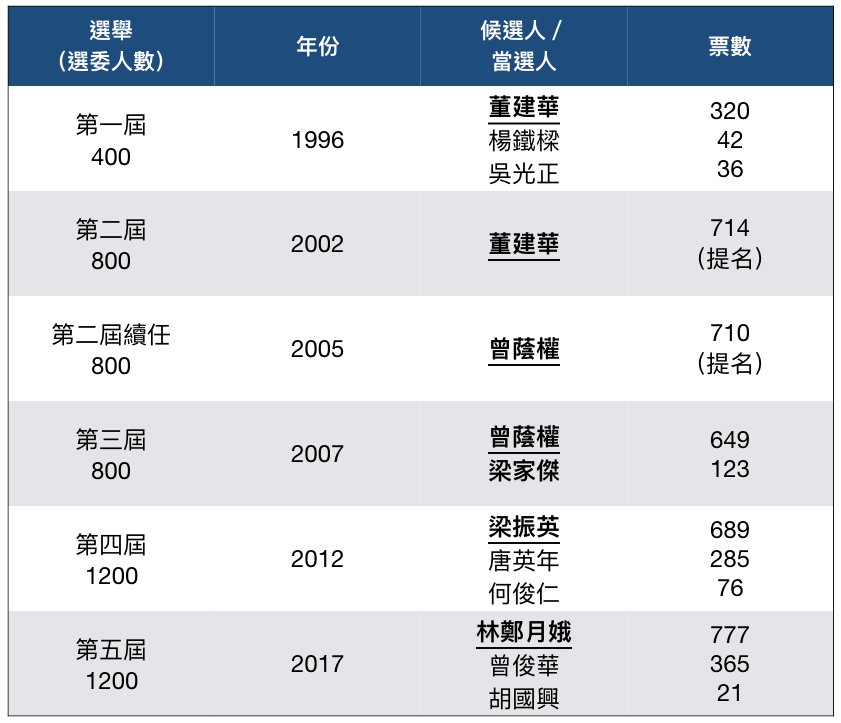
\includegraphics[width=0.7\textwidth]{c18/h-klesson1-026.png}
    \caption{特區成立以來的行政長官選舉結果} 
\end{figure}

雖然只有獲得中央政府支持的候選人才有可能當選成為行政長官,但建制派當中不同陣營仍會互相較勁,希望在競選的過程中得到好處。這點在二零一二年和二零一七年兩屆行政長官選舉中特為明顯,因為這兩屆競選都出現了多於一位被認為來自建制派的候選人。不過,這種內部競爭並沒有提高選舉的認授,反而更突顯其缺陷。

以林鄭月娥為例,她在鄉事問題的立場逆轉就被批為引證了「小圈子選舉」的缺陷。她在二零一一年擔任發展局局長時,曾經表明要嚴厲執法取締僭建村屋,甚至一度聲稱要終止新界原居民的「丁權」,引發鄉事勢力的強烈反彈,更有村民火燒其紙紮人像以示抗議。打擊村屋僭建問題後來不了了之,林鄭月娥到了二零一七年參選行政長官時更改稱「執法有緩急先後」,態度明顯改變。與此同時,鄉議局於選舉委員會的27票全數投與林鄭月娥,並呼籲其他來自新界鄉郊地區選委支持。外界評論普遍認為這是一次赤裸裸的利益交換,也突顯了候選人為了討好個別界別的利益,可以置全港整體利益不顧。

提到林鄭月娥,她的當選也打破了特區成立以來的一個共識:儘管行政長官不是由普選產生,但此前每屆的當選人都是當時最受市民支持的候選人,建制陣營仍可聲稱選舉委員會履行了普遍市民的意願。不過林鄭月娥雖然並非最受市民歡迎,卻得到大多數選委投票支持當選。按香港大學民意研究計劃所得,另一位候選人曾俊華於選舉前最後一後一輪的民意調查獲得52.8%的支持,遠遠拋離林鄭月娥所得的32.1%。至於接受程度方面,曾俊華的支持度淨值達59.8%,而林鄭月娥則為負7.5%,即反對她的受訪者被支持的還要多。也就是說,二零一七年行政長官的結果背離了民意依歸,被稱為假選舉亦不為過。



伸延閱讀:

楊艾文,高禮文(2011):《選舉香港特區行政長官》,香港:香港大學出版社。

Gittings D, 2016, Selecting the Chief Executive, \textit{Introduction to the Hong Kong Basic Law}